%%
%% ****** ljmsamp.tex 13.06.2018 ******
%%
\documentclass[
11pt,%
tightenlines,%
twoside,%
onecolumn,%
nofloats,%
nobibnotes,%
nofootinbib,%
superscriptaddress,%
noshowpacs,%
centertags]%
{revtex4}
\usepackage{ljm}
\begin{document}

\titlerunning{Short form of the title} % for running heads
\authorrunning{First-Author at al.} % for running heads
%\authorrunning{First-Author, Second-Author} % for running heads

\title{Title of the Article,\\
Broken into Lines}
% Splitting into lines is performed by the command \\
% The title is written in accordance with the rules of capitalization.

\author{\firstname{A.~A.}~\surname{First-Author}}
\email[E-mail: ]{First.Author@email.com}
\affiliation{Place of work and/or the address of the first and second authors}
\affiliation{Example: N.I. Lobachevskii Institute of Mathematics and Mechanics, Kazan (Volga Region) Federal University, Kremlevskaya ul. 18, Kazan, Tatarstan, 420008 Russia}

\author{\firstname{B.}~\surname{Second-Author}}
\email[E-mail: ]{Second.Author@email.com}
\affiliation{Place of work and/or the address of the first and second authors}
\affiliation{Place of work and/or the address of second authors}
%\noaffiliation % If the author does not specify a place of work.

\firstcollaboration{(Submitted by A.~A.~Editor-name)} % Add if you know submitter.
%\lastcollaboration{ }

\received{June 13, 2018} % The date of receipt to the editor, i.e. December 06, 2017


\begin{abstract} % You shouldn't use formulas and citations in the abstract.
In this example, the article contains some required author
information and examples of how to gain an article in the REV\TeX~4
for \ljm. You shouldn't use formulas and citations in the abstract.
\end{abstract}

\subclass{12345, 54321} % Enter 2010 Mathematics Subject Classification.

\keywords{Keyword1, Keyword2} % Include keywords separeted by comma.

\maketitle

% Text of article starts here.

\section{Introduction}

To prepare your manuscript, use REV\TeX{} package. The latest version can be downloaded at the project homepage \cite{RTeXHome}.
The process of processing an article using REV\TeX{} is described in detail in the package manuals \cite{RTeX}. Great help in resolving technical
issues on \TeX{} can be found in books \cite{texbook,L,GG,KD}.
Use the ``House Style Guide: Version 2.0'' \cite{hsg} for more help on how to format article.

\section{First level Heading\protect\\
broken into lines}

There are three levels of Headings that are set by the commands
\verb|\section|, \verb|\subsection|, and \verb|\subsubsection|
(Chapter, subchapter, subsection). Split header into lines
is done with the command \verb+\protect\\+.
Second level heading as the title of article is written in accordance with the rules of capitalization \cite{cap}.

\subsection{Second Level Heading}

References in the text are by using the commands
\verb+\cite{#1}+ or \verb+\onlinecite{#1}+. Label \verb+#1+
can have a name consisting of both letters and numbers. In
the bibliography section\footnote{See the end of the article.} this link also has a label \verb+#1+ and starts the command \verb+\bibitem{#1}+.

With the command \verb+\cite{texbook}+ get a reference \cite{texbook},
if you need to refer to several sources:
\cite{texbook,L}, the curly brackets indicate references
separated by commas: \verb+\cite{texbook,L}+. When
use the command \verb|\onlinecite{#1}| link will not be
in brackets: see~\onlinecite{texbook}, p.~8.
If there is a link to the sources with serial numbers,
e.g. [1,2,3,6,7,8], then print automatically following links will take
[1--3,6--8].

\section{Standalone formulae}

\subsection{Another second-level heading}

In \LaTeX, there are many ways to embed standalone formulas
on the page and align them. By default, formulas always
centered.

\subsubsection{One-line formulas}

Below are examples of one-line equations:
\begin{eqnarray}
\chi_+(p)\alt{\bf [}2|{\bf p}|(|{\bf p}|+p_z){\bf ]}^{-1/2}
\left(
\begin{array}{c}
|{\bf p}|+p_z\\
px+ip_y
\end{array}\right)\;,
\\
\left\{%
\openone234567890abc123\alpha\beta\gamma\delta1234556\alpha\beta
\frac{1\sum^{a}_{b}}{A^2}%
\right\}%
\label{one}.
\end{eqnarray}
The second formula has the number~(\ref{one}), which is set by command
\verb|\label{one}|. The first formula is assigned a number~(1), but
it cannot be applied with the help of automatic links,
as it has no label.

If the formula number is not necessary, use the environment
\verb+\[+, \verb+\]+, (or \$...\$) which obtained the following formula:
\[g^+g^+ \rightarrow g^+g^+g^+g^+ \dots ~,~~q^+q^+\rightarrow
q^+g^+g^+ \dots ~. \] % You also can use the dollar sign ($).

\subsubsection{Multiline formulae}

Multiline formulas are typed using the environment
eqnarray:
\begin{eqnarray}
{\cal M}=&&ig_Z^2(4E_1E_2)^{1/2}(l_i^2)^{-1}
\delta_{\sigma_1,-\sigma_2}
(g_{\sigma_2}^e)^2\chi_{-\sigma_2}(p_2)\nonumber\\
&&\times
[\epsilon_jl_i\epsilon_i]_{\sigma_1}\chi_{\sigma_1}(p_1),
\end{eqnarray}
\begin{eqnarray}
\sum \vert M^{\rm viol}_g \vert ^2&=&g^{2n-4}_S(Q^2)~N^{n-2}
(N^2-1)\nonumber \\
 & &\times \left( \sum_{i<j}\right)
\sum_{\rm perm}
\frac{1}{S_{12}}
\frac{1}{S_{12}}
\sum_\tau c^f_\tau~.
\end{eqnarray}
If the formula number is not necessary, then at the end of the row in front of the sign
\verb|\\| you need to put the command \verb|\nonumber|. Never
use one line command \verb|\nonumber| and
\verb|\label{#1}|, as this may cause error in automatic
the numbering of references.

If you want to gain a few formulas without number,
use the eqnarray environment* (the asterisk means the abolition
numbering):
\begin{eqnarray*}
\sum \vert M^{\rm viol}_g \vert ^2&=&g^{2n-4}_S(Q^2)~N^{n-2}
(N^2-1)\\
& &\times \left( \sum_{i<j}\right)
\left(
\sum_{\rm perm}\frac{1}{S_{12}S_{23}S_{n1}}
\right)
\frac{1}{S_{12}}~.
\end{eqnarray*}
To add numbers to the formula manually, use the command
\verb+\tag{#1}+, where \verb+#1+~--- the desired equation number.
Here how is the formula with the number of~(\ref{eq:mynum}):
\begin{equation}
g^+g^+ \rightarrow g^+g^+g^+g^+ \dots ~,~~q^+q^+\rightarrow
q^+g^+g^+ \dots ~. \tag{2.6$'$}\label{eq:mynum}
\end{equation}

When you enable single-line and multi-line formulas are surrounded by
subequations, each formula `numbered" with a letter,
as shown in equations~(\ref{mlett:1}) and (\ref{mlett:2}):
\begin{subequations}
\label{generallabel}
\begin{equation}
\left\{
abc123456abcdef\alpha\beta\gamma\delta1234556\alpha\beta
\frac{1\sum^{a}_{b}}{A^2}
\right\},\label{mlett:1}
\end{equation}
\begin{eqnarray}
{\cal M}=&&ig_Z^2(4E_1E_2)^{1/2}(l_i^2)^{-1}
(g_{\sigma_2}^e)^2\chi_{-\sigma_2}(p_2)\nonumber\\
&&\times
[\epsilon_i]_{\sigma_1}\chi_{\sigma_1}(p_1).\label{mlett:2}
\end{eqnarray}
\end{subequations}
If you put the label right after the \verb+\begin{subequations}+,
it can be used further as a reference to all the equations in this
environment. For example, you can refer to
equation~(\ref{generallabel}) this example.

To set multi-line formulas you can use the environment
multline, gather and align. The multline environment is good to use
for a set of standalone long formulas that do not fit on
one line:
\begin{multline}
\int_{a_1}^{a_2} f(x)\,dx+\int_{a_2}^{a_3} f(x)\,dx
+\dots+\int_{a_{n-1}}^{a_n} f(x)\,dx\\
+\int_{a_1}^{a_2} g(x)\,dx+\int_{a_2}^{a_3} g(x)\,dx
+\dots+\int_{a_{n-1}}^{a_n} g(x)\,dx\\
+\int_{a_1}^{a_2} h(x)\,dx+\int_{a_2}^{a_3} h(x)\,dx
+\dots+\int_{a_{n-1}}^{a_n} h(x)\,dx\\
=\int_{a_1}^{a_n} f(x)+g(x)+h(x)\,dx.
\end{multline}
This formula is automatically numbered, if the formula number is not
need, you have to use the environment multline*.

Environment gather centers included in the formula:
\begin{gather}
\int_{a_1}^{a_2} f(x)\,dx+\int_{a_2}^{a_3} f(x)\,dx
+\dots+\int_{a_{n-1}}^{a_n} f(x)\,dx\\
+\int_{a_1}^{a_2} g(x)\,dx+\int_{a_2}^{a_3} g(x)\,dx
+\dots+\int_{a_{n-1}}^{a_n} g(x)\,dx\notag\\
+\int_{a_1}^{a_2} h(x)\,dx+\int_{a_2}^{a_3} h(x)\,dx
+\dots+\int_{a_{n-1}}^{a_n} h(x)\,dx\\
=\int_{a_1}^{a_n} f(x)+g(x)+h(x)\,dx.
\end{gather}
Each line is automatically numbered, if the line number
it is not necessary, before \verb+\\+ in this line, you need to put the command
\verb+\notag+. When you use the environment gather* formula
will not be numbered.

The align environment allows you to align formulas on your
discretion:
\begin{align}
\int_{a_1}^{a_2} f(x)\,dx &+\int_{a_2}^{a_3} f(x)\,dx
+\dots+\int_{a_{n-1}}^{a_n} f(x)\,dx\notag\\
&+\int_{a_1}^{a_2} g(x)\,dx +\int_{a_2}^{a_3} g(x)\,dx
+\dots+\int_{a_{n-1}}^{a_n} g(x)\,dx\\
&+\int_{a_1}^{a_2} h(x)\,dx+\int_{a_2}^{a_3} h(x)\,dx
+\dots+\int_{a_{n-1}}^{a_n} h(x)\,dx\notag\\
&=\int_{a_1}^{a_n} f(x)+g(x)+h(x)\,dx.
\end{align}
Read more about working with these environments can be found in the book
\cite{GG}.

\section{Variables}
For the writing of definitions, theorems, lemmas and their proofs use the following variables. If necessary, you can add your variables in the sample.

\begin{definition}\label{D:1}
Define ...
\end{definition}

\begin{lemma}\label{L:1}
If ...
\end{lemma}

\begin{theorem}\label{Th:1}
Let ...
\end{theorem}
\begin{proof}
Consider...
\end{proof}

\section{Figures and tables}
REV\TeX~4 will automatically number sections, equations, tables, and
drawings. Figure captions are made after the image and the signature
tables~--- before a table, as shown in the examples at the end. In
tables footnotes \footnote{Footnotes in tables, you can try
to do this manually.} not working.

Graphics and diagrams should be monochrome in black-and-white color and saved in EPS format.
%You can include a picture in the article using the figure environment:
\begin{figure}[h]
\setcaptionmargin{5mm}
%\onelinecaptionsfalse % if the caption is multiline
\onelinecaptionstrue  % if the caption is one-line
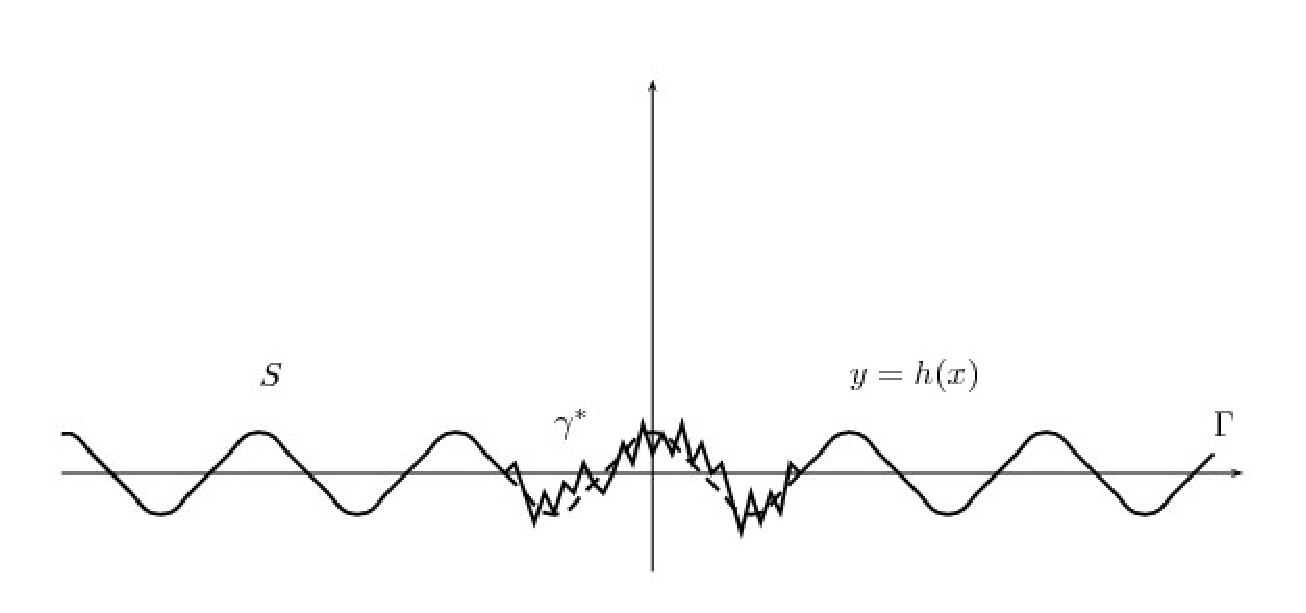
\includegraphics[width=0.85\textwidth]{deform.eps}
\captionstyle{normal}\caption{Please write your figure caption here.}\label{fig:1}
\end{figure}

\begin{table}[!h]
\setcaptionmargin{0mm}
\onelinecaptionsfalse
\captionstyle{flushleft}
\caption{ For the insertion of tables, the table environment is used,
 the signatures to the tables are made in the same way as the captions
 for the figures. This is an example of a table whose multi-line name
 is decorated with the \textbf{caption2} package.}
\bigskip
\begin{tabular}{|c|c|c|c|c|c|c|c|}
\hline
 &$r_c$ (\AA)&$r_0$ (\AA)&$\kappa r_0$&
 &$r_c$ (\AA) &$r_0$ (\AA)&$\kappa r_0$\\
\hline
Cu& 0.800 & 14.10 & 2.550 &Sn
& 0.680 & 1.870 & 3.700 \\
Ag& 0.990 & 15.90 & 2.710 &Pb
& 0.450 & 1.930 & 3.760 \\
Au& 1.150 & 15.90 & 2.710 &Ca
& 0.750 & 2.170 & 3.560 \\
Mg& 0.490 & 17.60 & 3.200 &Sr
& 0.900 & 2.370 & 3.720 \\
Zn& 0.300 & 15.20 & 2.970 &Li
& 0.380 & 1.730 & 2.830 \\
Cd& 0.530 & 17.10 & 3.160 &Na
& 0.760 & 2.110 & 3.120 \\
Hg& 0.550 & 17.80 & 3.220 &K &  1.120 & 2.620 & 3.480 \\
Al& 0.230 & 15.80 & 3.240 &Rb & 1.330 & 2.800 & 3.590 \\
Ga& 0.310 & 16.70 & 3.330 &Cs & 1.420 & 3.030 & 3.740 \\
In& 0.460 & 18.40 & 3.500 &Ba & 0.960 & 2.460 & 3.780 \\
Tl& 0.480 & 18.90 & 3.550 & & & & \\[1mm]
\hline
\end{tabular}
\end{table}

\begin{table}[!htb]
\setcaptionmargin{0mm}
\onelinecaptionstrue
\captionstyle{flushleft}
\caption{The name of this table is --- one-line.}
\bigskip
\begin{tabular}{|c|c|c|c|c|c|c|}
  \hline
    & 1 & 2 & 3 & 4 & 5 & 6\\
  \hline
  1 & 1 & 2 & 3 & 4 & 5 & 6\\
  2 & 2 & 4 & 6 & 8 & 10 & 12\\
  3 & 3 & 6 & 9 & 12 & 15 & 18\\[1mm]
  \hline
\end{tabular}
\end{table}

\section{Bibliography}
The following rules apply for references to books:

\begin{itemize}
  \item Author�s initials go before the surname with a space between the initials. Use and between the last two authors. All authors listed in the original reference should be cited.
  \item The title of the book is written in italics. If the book is originally published in Russian, only the English translation of the title is cited and after citation the original language may be indicated in square brackets, e.g.: [in Russian].
  \item Examples of bibliographic references can be found at the end of this page (i.e. article \cite{ex}, PhD thesis \cite{maguire-76}).
\end{itemize}


\begin{acknowledgments}
At the end of the articles are written thanks.\\
For example:\\
We thank A.~A.~Surname1 and B.~B.~Surname2 for their participation in discussions of the results.\\
We are grateful to C.~C.~Surname3 and the reviewers for careful reading of the manuscript and helpful remarks.

Links to grants are also listed here.
\end{acknowledgments}

% Text of article ends here.

\appendix

\section{Applications}

To switch to the tab application, you need to use the command
\verb+\appendix+. After all the sections will be referred to the word
The application and the corresponding letter in the command \verb+\section+
you don't specify, then the application will have
names.

\section{}

The application may contain subchapters and subsections.


%
% The Bibliography
%

\begin{thebibliography}{99}
\bibitem{RTeXHome}
\refitem{misc}
REV\TeX Home Page. \url{https://journals.aps.org/revtex}. Accessed 2018.

\bibitem{RTeX}
\refitem{manual}
REV\TeX~4.1 Author's Guide, American Physical Society, Research Road, Ridge, NY 11961 (2010). \url{https://d22izw7byeupn1.cloudfront.net/files/revtex/auguide4-1.pdf}. Accessed 2018.

\bibitem{texbook}
\refitem{book}
D.~E. Knuth, \emph{The TeXbook} (Addison-Wesley, London, 1984).

\bibitem{L}
\refitem{book}
S.~M. L'vovskij, \emph{Nabor i verstka v pakete \LaTeX, 2-e izdanie} (Kosmosinform, Moscow, 1995) [in Russian].

\bibitem{GG}
\refitem{book}
G.~Grjetcer, \emph{Pervye shagi v \LaTeX'e} (Mir, Moscow, 2000) [in Russian].

\bibitem{KD}
\refitem{book}
H.~Kopka and P.~Daly, \emph{A Guide to \LaTeXe} (Addison-Wesley, Reading, MA, 1995).

\bibitem{hsg}
\refitem{misc}
House Style Guide: Version 2.0. \url{http://ojs.kpfu.ru/files/HSG2013.pdf}. Accessed 2018.

\bibitem{cap}
\refitem{misc}
J. Frost, Capitalization in Titles 101. \url{https://www.grammarcheck.net/capitalization-in-titles-101}. Accessed 2018.

\bibitem{ex}
\refitem{article}
N.~Firstname and N.~Secondname, \textquotedblleft Title of article example,\textquotedblright Journal title \textbf{3}
  (12), 1--3 (2018).

\bibitem{maguire-76}
\refitem{phdthesis}
A.~Surname, Ph.d. diss., Department of Mathematics, University, Kazan (2018).

\end{thebibliography}
\end{document}
